\chapter{Time Management and Cost Estimate}
We now briefly describe the multiple stages of this project, along with their corespondent time constraints and associated cost. By the end of this chapter, we will have a rough idea of the total time needed to carry out the project as well as an estimate for its total monetary cost.

The chapter will be broken down into two main sections. The first one will focus on the time aspect of the project, while the second one will address the cost.

In regard to estimating the cost, it will be broken down into two groups.
\begin{itemize}
    \item \textbf{Human resources}. Very rough estimate of the amount of work hours needed for each person involved, along with the total cost when computing in the value for each hour and for each person.
    \item \textbf{Hardware and software}. Cost of the equipment needed as well as any non-free software used.
\end{itemize}

\section{Time Management}
In this section, we will attempt to calculate how long will this project take. Afterwards, a Gantt chart, Figure \ref{fig:gantt_chart}, visualizes the time cost for each development stage. For the begin and end date of each stage, refer to Table \ref{tab:gantt_dates}.

Moreover, this estimation is done prior to starting the project. It may or may not correspond to the actual amount time the project required. The main goal of this section is to have a point of reference we can fall back during the realization of the project.

With that in mind, here we enumerate every development stage with a significant time cost.
\begin{itemize}
    \item \textbf{State of the Art revision}. A study of the already existing solutions is necessary in order to choose the most suitable one.
    \item \textbf{Testing Environment Setup}. Since we lack a physical network for testing, we need to set up a robust virtual environment. 
    \item \textbf{Implementation}. Once the testing environment is ready, we can begin to configure FlowVisor.
    \item \textbf{Testing}. We make sure the hypervisor works as expected and the configuration is correct.
    \item \textbf{Documentation}. This is technically not a stage, as it spans the entire duration of the project. It is also not tied to any other stage in particular, so it can be done in parallel.
\end{itemize}

\begin{figure}
  \centering
  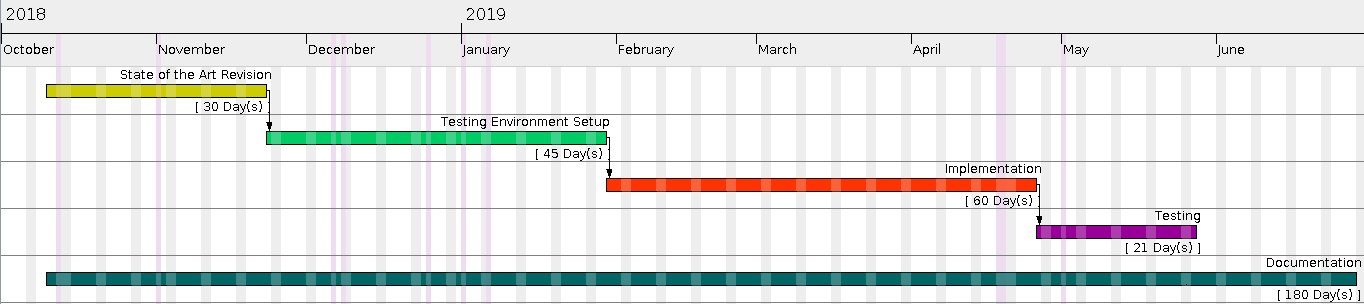
\includegraphics[width=\linewidth]{imagenes/TimeCost/Gantt_chart.png}
  \caption{Gantt Chart.}
  \label{fig:gantt_chart}
\end{figure}

\begin{table}
    \centering
    \caption{Duration, begin date and end date for each development stage.}
    \vspace{0.1 cm}
    \begin{tabular}{l c c c}
    \hline
    \rowcolor{lightgray}
    \textbf{Development stage}           &\textbf{Duration} &\textbf{Start}   &\textbf{End}            \\ \hline
    State of the art revision            & 25 days          & 10/10/2018      & 22/11/2018             \\ \hline 
    Environment Setup                    & 45 days          & 23/11/2018      & 29/01/2019             \\ \hline
    Implementation			             & 60 days          & 30/01/2019      & 25/04/2019             \\ \hline
    Testing          		             & 21 days          & 26/04/2019      & 27/05/2019             \\ \hline
    Documentation			             & 183 days         & 10/10/2018      & 28/06/2019             \\ \hline
    \end{tabular}
    \label{tab:gantt_dates}
\end{table}

From this data, we estimate this project's length to span over 183 days. This is the duration of the documentation stage, as we consider it to be the bottleneck.

\section{Cost Estimate}
This section will cover the estimation of the budget necessary to carry out the present project. Moreover, it is not the intent of this section to provide a very accurate answer. On the contrary, the actual purpose is just to obtain an approximate cost that would be within the same order of magnitude of the actual cost if it were possible to compute.

Furthermore, to make the estimate geographically agnostic, prices will not include VAT nor shipping cost when applicable.

\subsection{Human Resources}
The following people have worked or contributed to this project in one way or another:
\begin{itemize}
    \item \textbf{Jorge Navarro-Ortiz}. Associate professor of the Department of Signal Theory, Telematics and Communications of the University of Granada, as thesis supervisor.
    \item \textbf{Angel Guzman-Martinez}. Student of the School of Informatics and Telecommunications Engineering of the University of Granada.
\end{itemize}

Currently in Spain, disclosing a salary/price of reference for any profession or service is forbidden by law \cite{spanish_government_defensa_2007}. Therefore, this category will be based on the assumption that a telecommunication engineer, usually earns no less than \EUR{20} per hour and no more than \EUR{50} per hour. From there, we have decided to assign \EUR{25}/h to Angel Guzman-Martinez and \EUR{50}/h to Jorge Navarro-Ortiz.

In order to compute the actual cost for each person, we also need to estimate the amount of hours contributed towards the project. Again, this will be just an approximation.

\begin{itemize}
\item Angel Guzman-Martinez: 3 hours a day during 9 months excluding weekends. This yields, approximately, \textbf{594 hours.}
\item Jorge Navarro-Ortiz: \textbf{8 hours} in total of tutorship.
\end{itemize}

Taking everything into account, the total cost for human resources amounts to \textbf{\EUR{15,250}}. Refer to Table \ref{tab:HumanResources} for a quick summary.

\begin{table}
    \centering
    \caption{Human resources cost.}
    \vspace{0.1 cm}
    \begin{tabular}{l c c c}
    \hline
    \rowcolor{lightgray} \textbf{Concept}&\textbf{Cost/time}&\textbf{Quantity}&\textbf{Total}          \\ \hline
    Project work		  	             & \EUR{25}/h       & 594 hours       & \EUR{14,850}           \\ \hline 
    Tutorship				             & \EUR{50}/h       & 8 hours         & \EUR{400}              \\ \hline
    \textbf{Total}				         &                  &                 & \textbf{\EUR{15,250}}  \\ \hline 
    \end{tabular}
    \label{tab:HumanResources}
\end{table}

\subsection{Mandatory Hardware and Software}
It is important to note that, in this section, we will only list the hardware and software strictly necessary for the project to work. Whatever was used exclusively for the testing phase will be addressed later in this chapter. With that said, here is the list of critical components:

\begin{itemize}
    \item \textbf{Laptop.} The physical platform that will host the Mininet virtual machine. Any laptop that is able to run virtualization software will do. In our case we use HP 250 G6 Notebook with an Intel i5-7200U CPU, an Intel HD Graphics 620 integrated GPU and 8GB of RAM.
    
    \item \textbf{GNU/Linux}. Our operative system of choice and it is free. In particular, we use the Arch Linux distribution with the Linux kernel version 5.1.3. There are many others free  distributions, as well as a paid alternative, i.e., Windows. Any of them would work just fine as long as they are able to run some kind of operative system virtualization.
    
    \item \textbf{Virtual Box.} Software used for operative system virtualization. Virtualbox is what we used for this project in order to deploy the Mininet virtual machine, but there are a few alternatives, e.g., QEMU or VMware. 
    
    We could also use Mininet natively if we already have a GNU/Linux installation, yet it is still beneficial to use the standalone virtual machine as it provides a custom kernel optimized towards network virtualization.
    
    \item \textbf{Mininet.} Framework that allows us to create a virtual network within a single device. Ideally, in an real scenario, a physical network would be used. However, we did not have that possibility, so the budget estimate will be based on what we have actually used.
    
    \item \textbf{FlowVisor.} Open source SDN hypervisor used for network slicing.
\end{itemize}

Thankfully, all of the software we need is open source and free for personal use, see Table \ref{tab:software}. In the case of Virtual Box, a license is required for commercial use, which is not our case.

As for the hardware, see \ref{tab:hardware}.

\begin{table}
    \centering
    \caption{Mandatory Hardware cost.}
    \vspace{0.1 cm}
    \begin{tabular}{l c c c c c}
    \hline
    \rowcolor{lightgray}
    \textbf{Concept}&\textbf{Unit cost}&\textbf{Units} &\textbf{Average lifespan}&\textbf{Time used} &\textbf{Total}     \\ \hline
    Laptop          & \EUR{700}        & 1             & 3 years                 & 183 days          &\EUR{117}          \\ \hline
    \textbf{Total}  &                  &               &                         &                   &\textbf{\EUR{117}} \\ \hline 
    \end{tabular}
    \label{tab:hardware}
\end{table}

\begin{table}
    \centering
    \caption{Mandatory Software cost.}
    \vspace{0.1 cm}
    \begin{tabular}{l c c c}
    \hline
    \rowcolor{lightgray}
    \textbf{Software}&\textbf{Open source}&\textbf{Free for personal use} &\textbf{License cost}             \\ \hline
    Virtual Box      & Yes                & Yes    			  	          &\EUR{0}                           \\ \hline 
    Mininet          & Yes                & Yes    			  	          &\EUR{0}                           \\ \hline 
    FlowVisor        & Yes                & Yes    			  	          &\EUR{0}                           \\ \hline 
    \textbf{Total}   &                    &                          	  &\textbf{\EUR{0}}                  \\ \hline 
    \end{tabular}
    \label{tab:software}
\end{table}

\subsection{Hardware and Software Used for Testing}
This section is included for completeness, and it will list everything that was used exclusively for testing. It is worth noting that there are plenty of alternatives as to how we have performed the testing, so that it is not necessary to use the same elements that are shown here.
\begin{itemize}
    \item \textbf{Raspberry Pi}. Used as external physical host. To be more specific, we will use a model 3B running the Raspbian operative system and kernel Linux 4.9.69-v7+. 
    
    \item \textbf{LoRa mote}. It will be tasked to periodically send LoRa packets. The exact model is TTGO LoRa32 V2.1\_1.6.
    
    \item \textbf{LoRa gateway}. Its purpose is to receive the LoRa packets and forward them through our Mininet network and towards a physical external host. The model we will use is called LoRa Lite Gateway, developed by IMST.
\end{itemize}

Note how there is no specific software used exclusively for testing, so everything will be summarized in Table \ref{tab:testing_hardware}.

\begin{table}
    \centering
    \caption{Testing Hardware cost.}
    \vspace{0.1 cm}
    \begin{tabular}{l c c c}
    \hline
    \rowcolor{lightgray}
    \textbf{Concept}&\textbf{Unit cost}&\textbf{Units}              &\textbf{Total}         \\ \hline
    Raspberry Pi    &\EUR{33.94}       & 1 	                        &\EUR{33.94}            \\ \hline 
    LoRa mote       &\EUR{18.84}       & 1 	                        &\EUR{18.84}            \\ \hline 
    LoRa gateway    &\EUR{199}         & 1 	                        &\EUR{199}              \\ \hline 
    \textbf{Total}  &                  &                            &\textbf{\EUR{251.78}}  \\ \hline 
    \end{tabular}
    \label{tab:testing_hardware}
\end{table}

\subsection{Total Cost}
Lastly, we present two different budget estimates.
\begin{itemize}
    \item \textbf{Only mandatory components}. A cheaper alternative that dismisses anything that is not strictly necessary for the project to work, Table \ref{tab:mandatory_budget}.
    \item \textbf{Complete budget}. Includes the mandatory components as well as the hardware and software that was used exclusively for testing, Table \ref{tab:complete_budget}.
\end{itemize}

\begin{table}[H]
    \centering
    \caption{Mandatory budget.}
    \vspace{0.1 cm}
    \begin{tabular}{l c c c}
    \hline
    \rowcolor{lightgray} \textbf{Concept}  &\textbf{Cost}               \\ \hline
    Human resources                        &\EUR{15,250}                \\ \hline 
    Hardware						       &\EUR{117}                   \\ \hline 	
    Software                               &\EUR{0}                     \\ \hline
    \textbf{Total}                         &\textbf{\EUR{15,367}}       \\ \hline   
    \end{tabular}
    \label{tab:mandatory_budget}
\end{table}

\begin{table}[H]
    \centering
    \caption{Complete budget.}
    \vspace{0.1 cm}
    \begin{tabular}{l c c c}
    \hline
    \rowcolor{lightgray} \textbf{Concept}  &\textbf{Cost}               \\ \hline
    Human resources                        &\EUR{15,250}                \\ \hline 
    Mandatory Hardware					   &\EUR{117}                   \\ \hline 	
    Testing Hardware					   &\EUR{251.78}                \\ \hline 	
    Software                               &\EUR{0}                     \\ \hline
    \textbf{Total}                         &\textbf{\EUR{15,618.78}}    \\ \hline   
    \end{tabular}
    \label{tab:complete_budget}
\end{table}

If we only take into account the mandatory assets, this project will need, approximately, a budget of \textbf{\EUR{15,367}}. 

\bigskip

On the other hand, if we include everything then we have an approximate cost of \textbf{\EUR{15,618.78}}.